\section{Introduction}
\label{sec:generalisation_intro}
Work is currently unpublished but is aiming to be submitted to the British Journal of Dermatology for publication. This work will be co-authored by Gillian Chin, Charlotte Proby, Emanuele Trucco, Colin Fleming and Stephen McKenna.

Dermatological classification of skin lesion images using deep learning (DL) has made considerable progress in recent years (Du‐Harpur et al.2020, Wu 2022). DL classifiers have proven effective with large datasets, several of which, most notably the ISIC archive, have enabled substantial progress (Tschandl 2018; Wen et al 2022). Some studies using high-quality datasets have reported performance matching or surpassing dermatologists (Esteva 2017; Haenssle 2018; Han 2018; Tschandl 2019). Studies have also investigated the ability of DL classifiers with macroscopic clinical images (Fujisawa et al. 2019). In contrast to dermoscopy images, community-acquired ones are of variable quality, with fields of view wider and less consistent than those of dermoscopic images. There are also often visual distractors present in these images.

Current DL classifiers for medical images can generalize poorly across healthcare systems, acquisition protocols, and populations. Evaluations reported in the literature are usually, though not always (e.g., Han et al. 2018), internal, with model training and testing datasets drawn from the same source. Questions remain over their ability to generalise across domains, data sets and cameras. Rather than aiming to develop a universally applicable skin lesion classifier, a more realistic approach envisages the use of local datasets to adapt models to target populations and systems XXX REF NEEDED. 

Labelled datasets can be expensive to create and curate (Chin et al. 2022), so domain knowledge acquired from large datasets from other domains needs to be transferred and brought to bear. Transfer learning XXX REF NEEDED can enable reuse of information learned from one domain (source) in another domain (target). Transfer learning is often used in medical image analysis due to limitations on dataset size, enabling features learned from large datasets to be fine-tuned for re-use in a target domain with smaller datasets. The extent to which transfer learning is beneficial also depends on the similarity of the source and target domains, as well as on the DL models used (Matsoukas et al. 2022); for example, transfer from the large ImageNet dataset (Deng et al. 2009) has been widely adopted in medical image analysis despite its visual dissimilarity to medical images. Specifically, deep classification of the ISIC 2019 dermoscopy dataset is known to benefit from transfer learning from ImageNet with evidence for feature re-use in this case (Matsoukas et al. 2022). 

In this paper, we investigate the extent to which transfer between dermatology datasets (after ImageNet pre-training) can be effective, using two types of DL model with different inductive biases. We expect effectiveness to depend on the size of source datasets used for pre-training, and on their similarity to the target datasets. XXX And what do we find?

Our focus is on the use of DL to assist diagnosis based on community images acquired with limited control. The performance of any DL algorithm will depend on the case mix within the training and testing groups. It is therefore critical to obtain data from the specific real-world setting in which the DL will be deployed. One important use case in UK dermatology is the image referrals sent to secondary-care hospital-based dermatologists from primary care. this was therefore selected as the use case for gathering, training and testing two novel datasets, intended for triage experiments with a DL system aiming to reliably identify common benign conditions in a real-world clinical setting, one where images were acquired in primary care and a comparator where referred images were sent for medical photography. 



\section{Generalisation Review}
\label{sec:generalisation_review}
Review



\section{Datasets}
\label{sec:generalisation_datasets}
We curated two datasets of community-acquired macroscopic (non-dermoscopic) images. These datasets were extracted from previously stored NHS images referred from primary to secondary care in Tayside, UK~\footnote{NHS Tayside: \url{nhstayside.scot.nhs.uk}} and Forth Valley, UK~\footnote{NHS Forth Valley: \url{nhsforthvalley.com}}.

\subsection{Tayside Dataset}
\label{subsec:tayside_dataset}
The Tayside images had been acquired by primary care practitioners using a variety of cameras, from all cutaneous anatomical sites, using non-standardised lighting, framing, focusing and acquisition setting. After cleaning (removal of duplicates and images not of clinical use, e.g., scanned written documents), data were cross-linked with the electronic patient record to determine the final diagnosis for the images. NHS Tayside has an in-house diagnostic database, Dermabase, wherein all patient contacts are mandated to have a consultant-level diagnostic label, using the BAD diagnostic index which corresponds to ICD-10. These were then de-identified manually and cropped to highlight abnormalities if required. Image labelling was done by four clinicians, including a consultant (CF) who had final decision on all diagnoses, thus producing a database of dermatology images defined by a consultant as well as diagnoses reviewed by a consultant.

\subsection{Forth Valley Dataset}
\label{subsec:forth_valley_dataset}
Forth Valley Data

\subsection{Annotation Procedure}
\label{subsec:annotation_procedure}
Annotation Procedure



\section{Generalisation Experiments}
\label{sec:generalisation_experiments}
This section details the datasets, training parameters, experimental setup, and results for the experiments with dermatology dataset cross generalisation. The code and full results used within this section can be found on the project GitHub repository~\footnote{GitHub Repository: \url{github.com/UoD-CVIP/Lesion-Classifier}}.

\subsection{Datasets}
\label{subsec:generalisation_datasets}
Images from two public domain skin lesion datasets were used in our experiments in addition to the datasets from Tayside and Forth Valley: the ISIC 2019 dataset~\citep{codella2018skin,combalia2019bcn20000,tschandl2018ham10000} and the SD-260 dataset~\citep{yang2019self}. The ISIC datasets are the largest publicly available, with ISIC 2019 containing over 26,000 skin lesion images labelled with diagnoses. Those images were acquired using dermatoscopes; they tend to be well-centred, zoomed in and of consistent resolution. SD-260 images were acquired in less controlled environments with varying imaging devices; hence, they vary more than the ISIC 2019 ones in colour, exposure, illumination, resolution, and scale. Visually they are qualitatively like the Tayside and Forth Valley datasets, but acquired from a Chinese population.

\begin{figure}
	\centering
	\captionsetup[subfigure]{singlelinecheck=false}
	\begin{tabular}{cc}
		\subcaptionbox{\centering Melanoma}{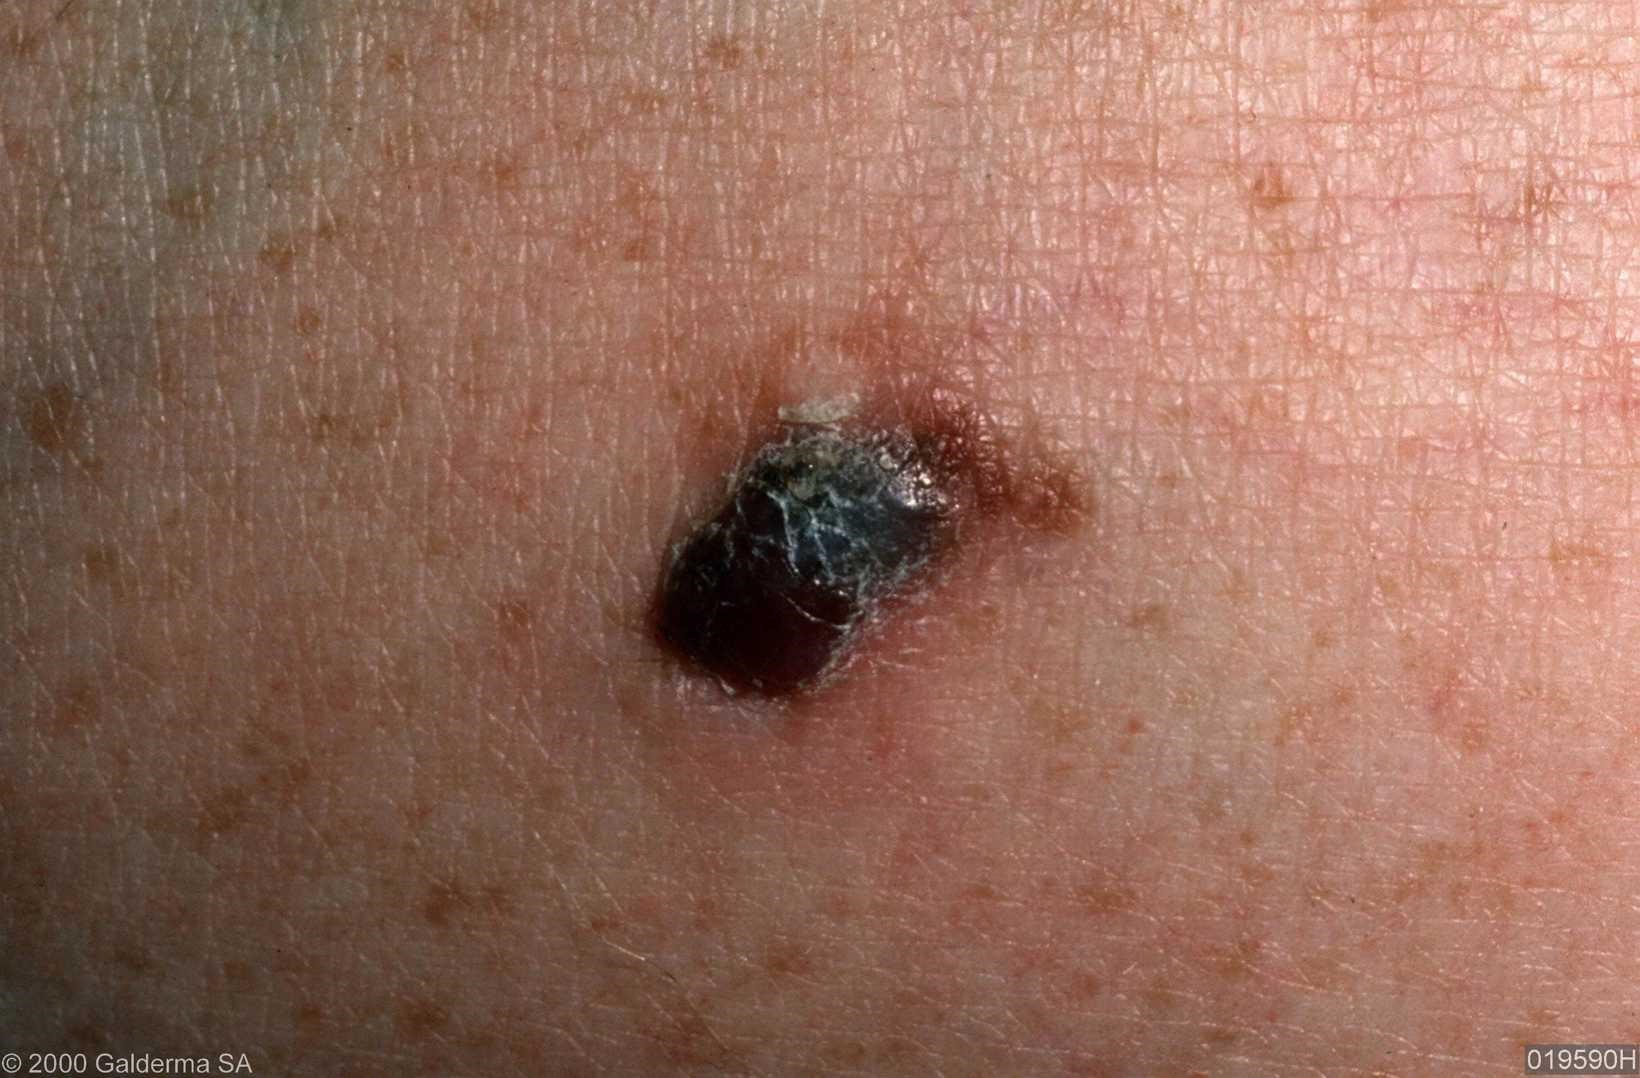
\includegraphics[width=0.45\textwidth]{images/sd260_mel.jpg}} &
		\subcaptionbox{\centering Melanocytic \mbox{Nevus}}{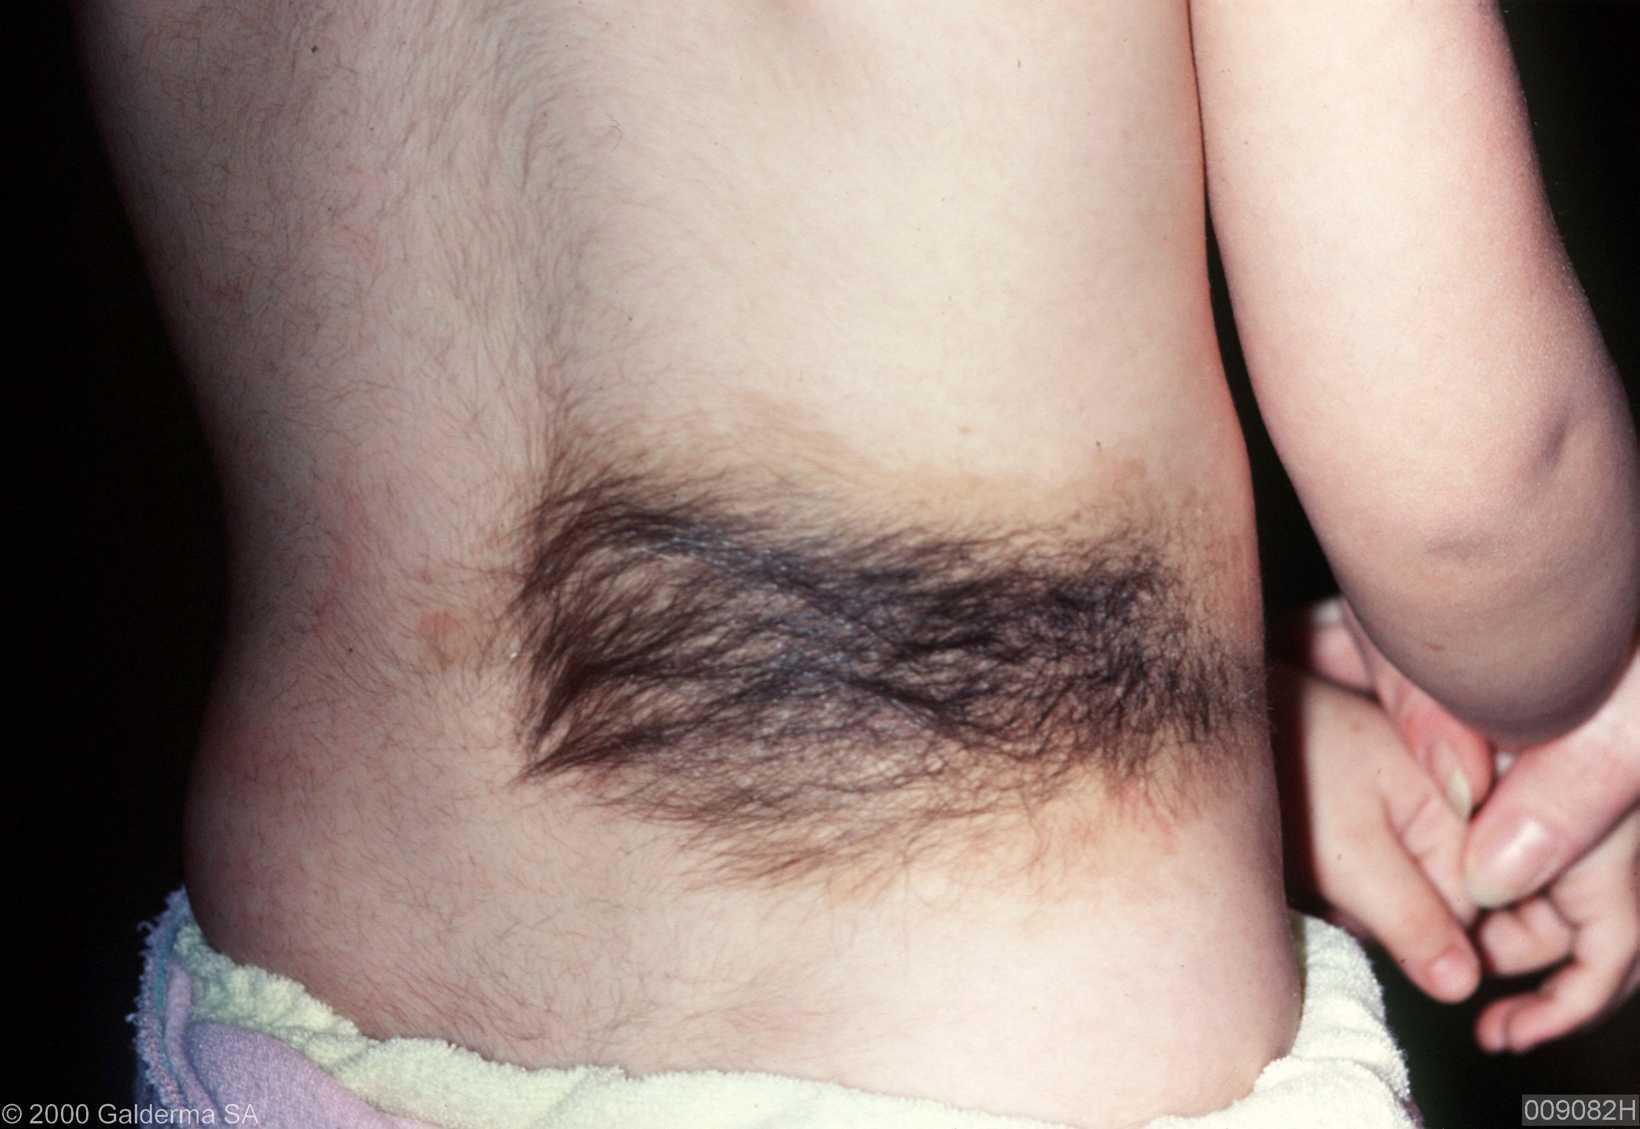
\includegraphics[width=0.45\textwidth]{images/sd260_nv.jpg}} \\
		\subcaptionbox{\centering Basal Cell \mbox{Carcinoma}}{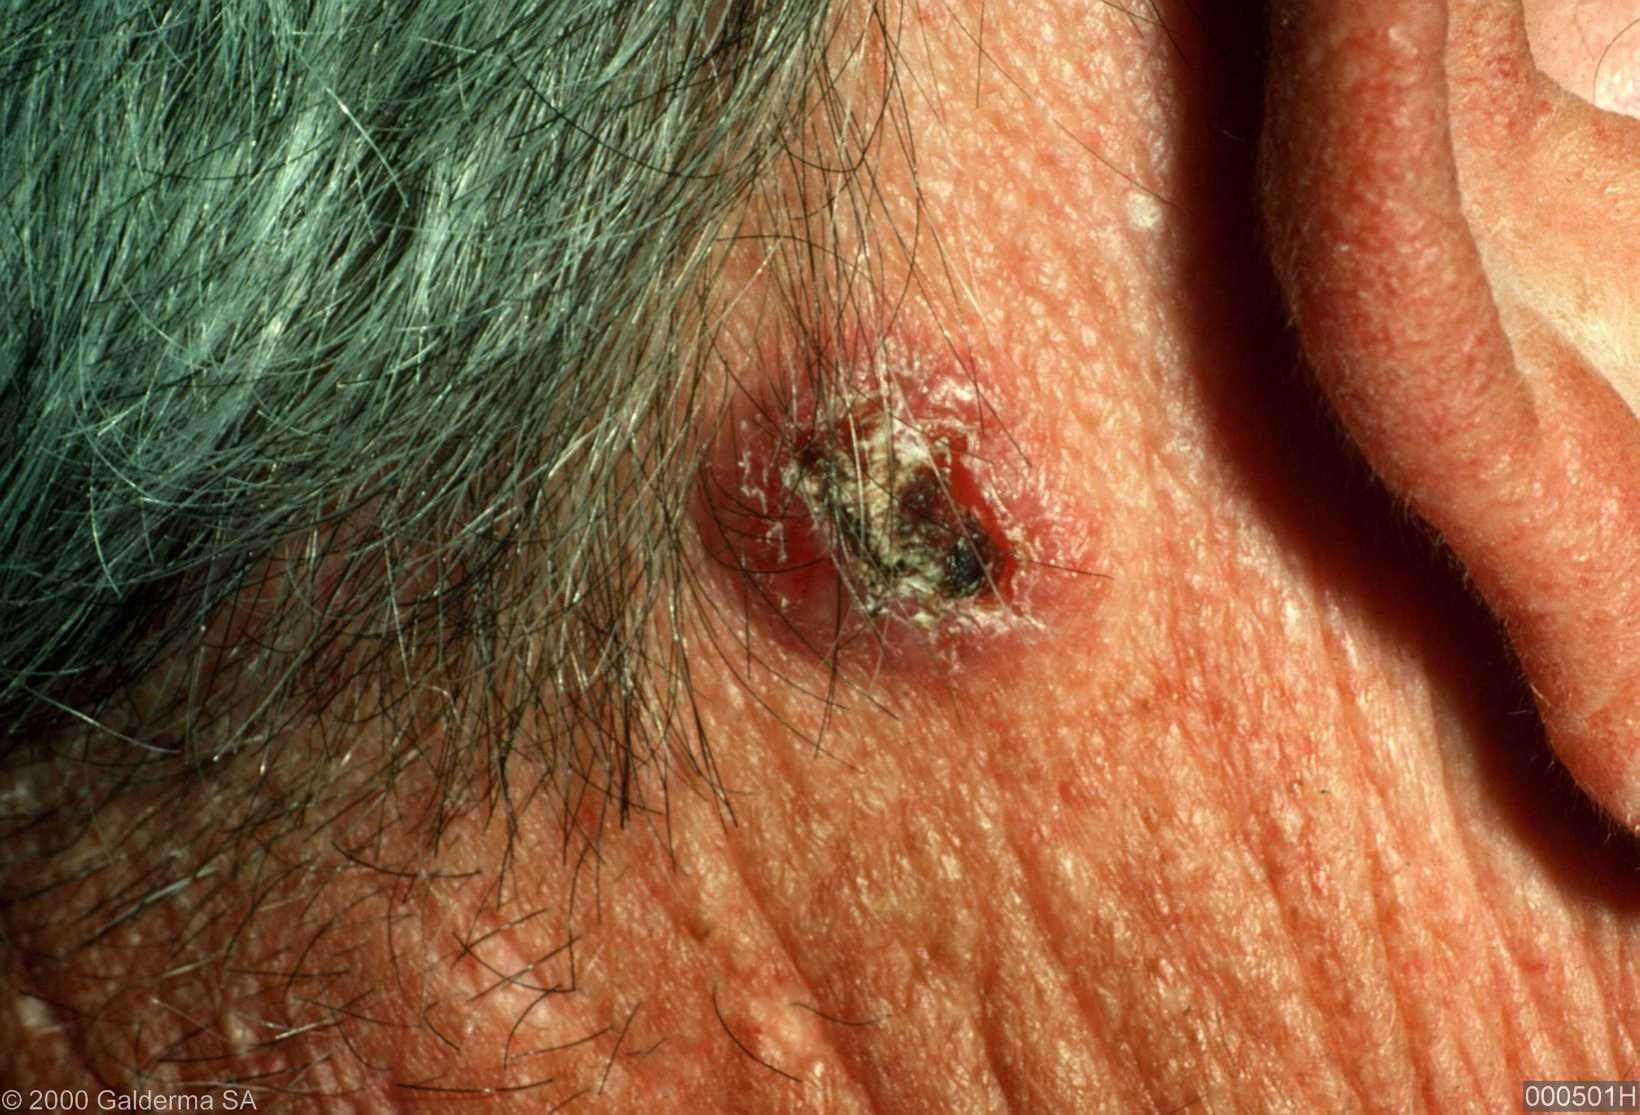
\includegraphics[width=0.45\textwidth]{images/sd260_bcc.jpg}} &
		\subcaptionbox{\centering Actinic Keratosis}{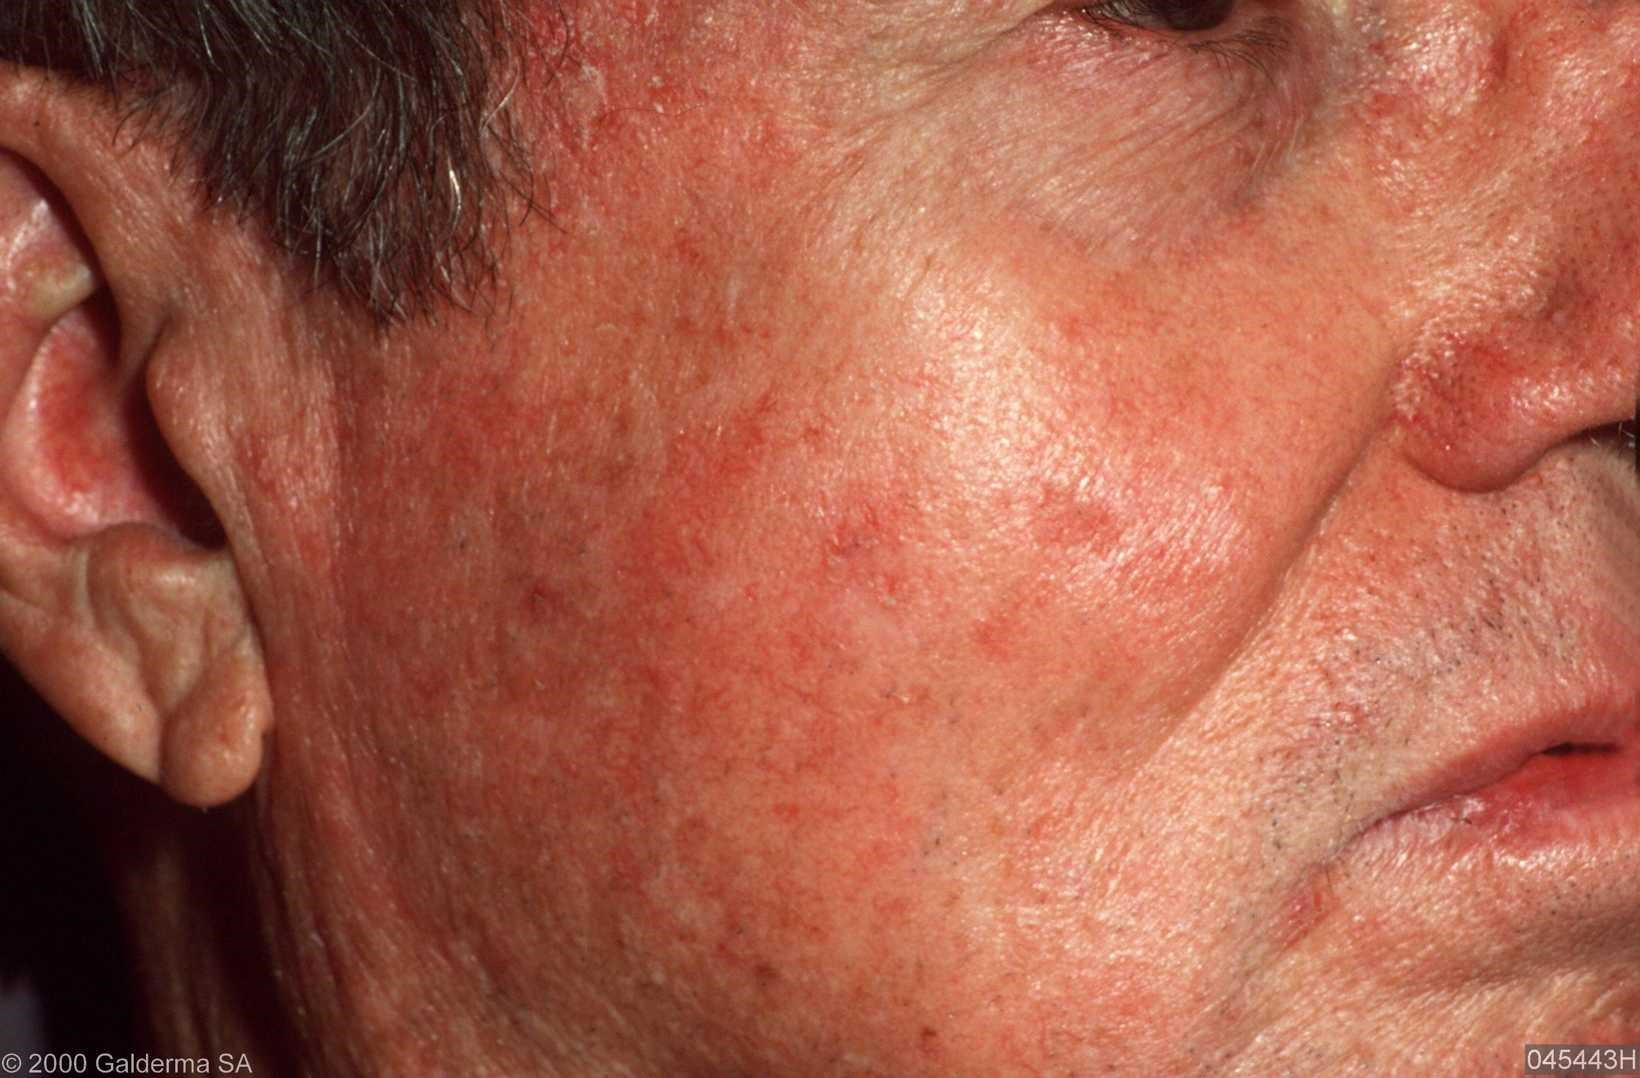
\includegraphics[width=0.45\textwidth]{images/sd260_ak.jpg}} \\
		\subcaptionbox{\centering Benign Keratosis}{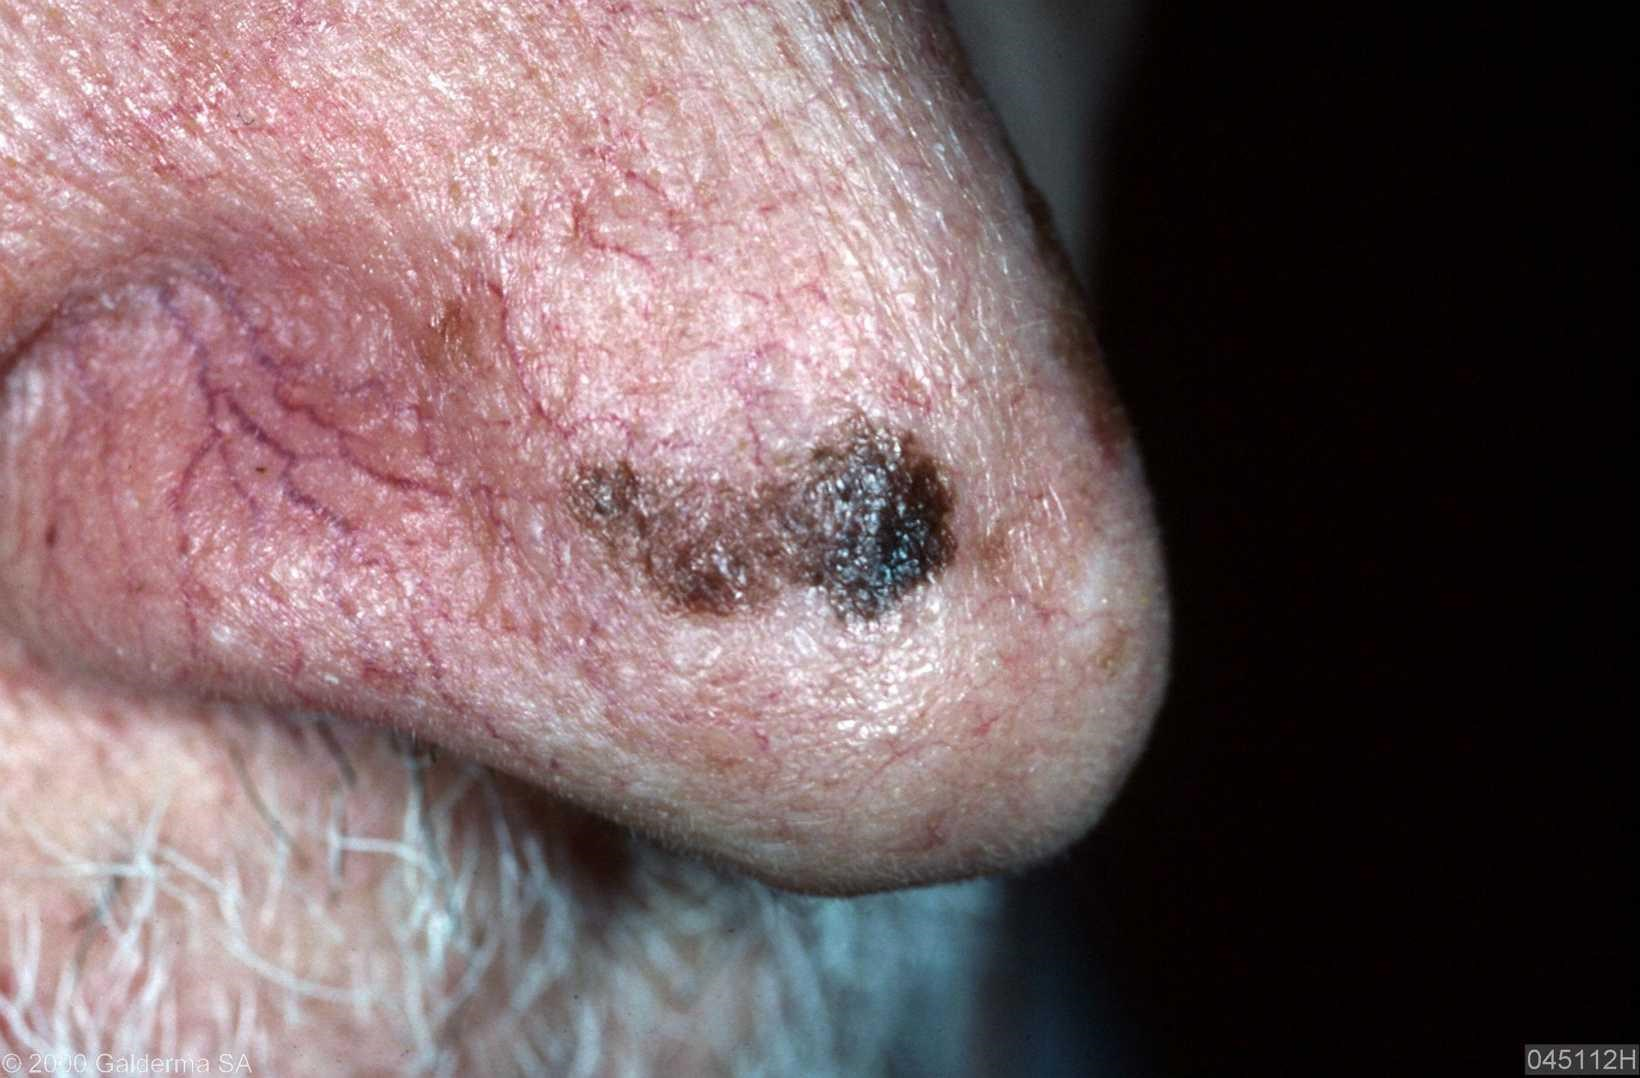
\includegraphics[width=0.45\textwidth]{images/sd260_bkl.jpg}} &
		\subcaptionbox{\centering Dermatofibroma}{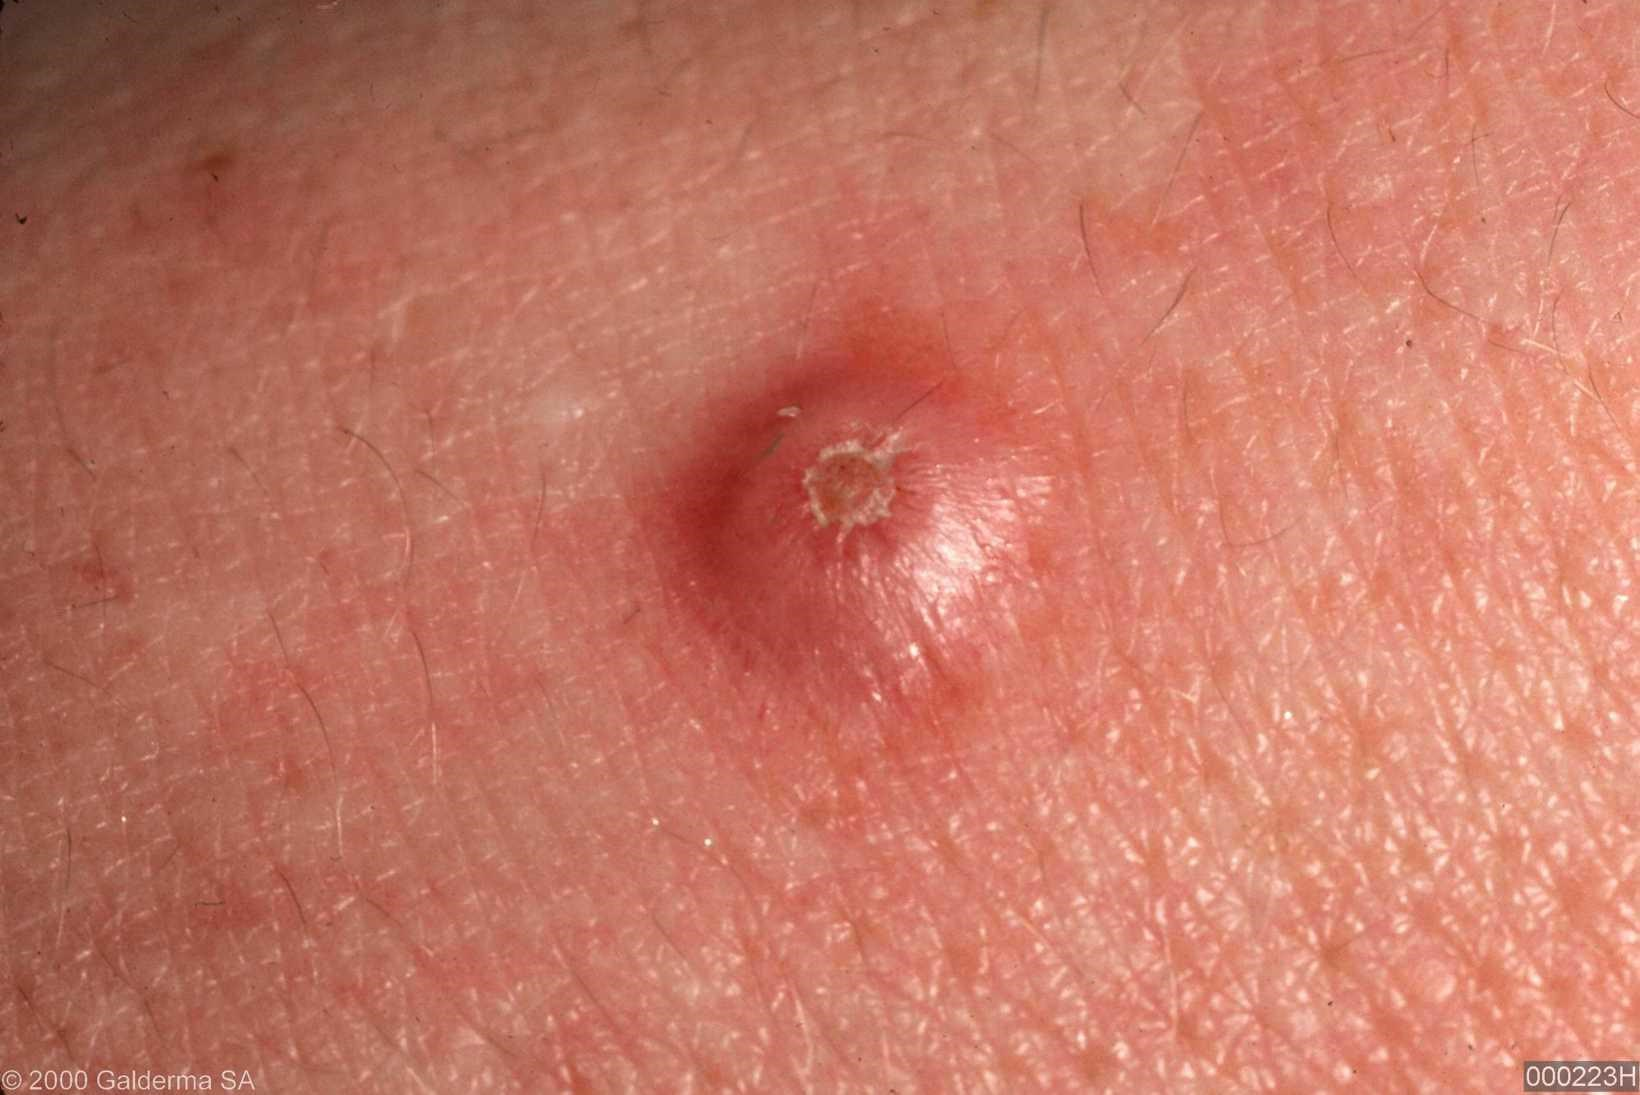
\includegraphics[width=0.45\textwidth]{images/sd260_df.jpg}} \\
		\multicolumn{2}{c}{\subcaptionbox{\centering Squamous Cell \mbox{Carcinoma}}{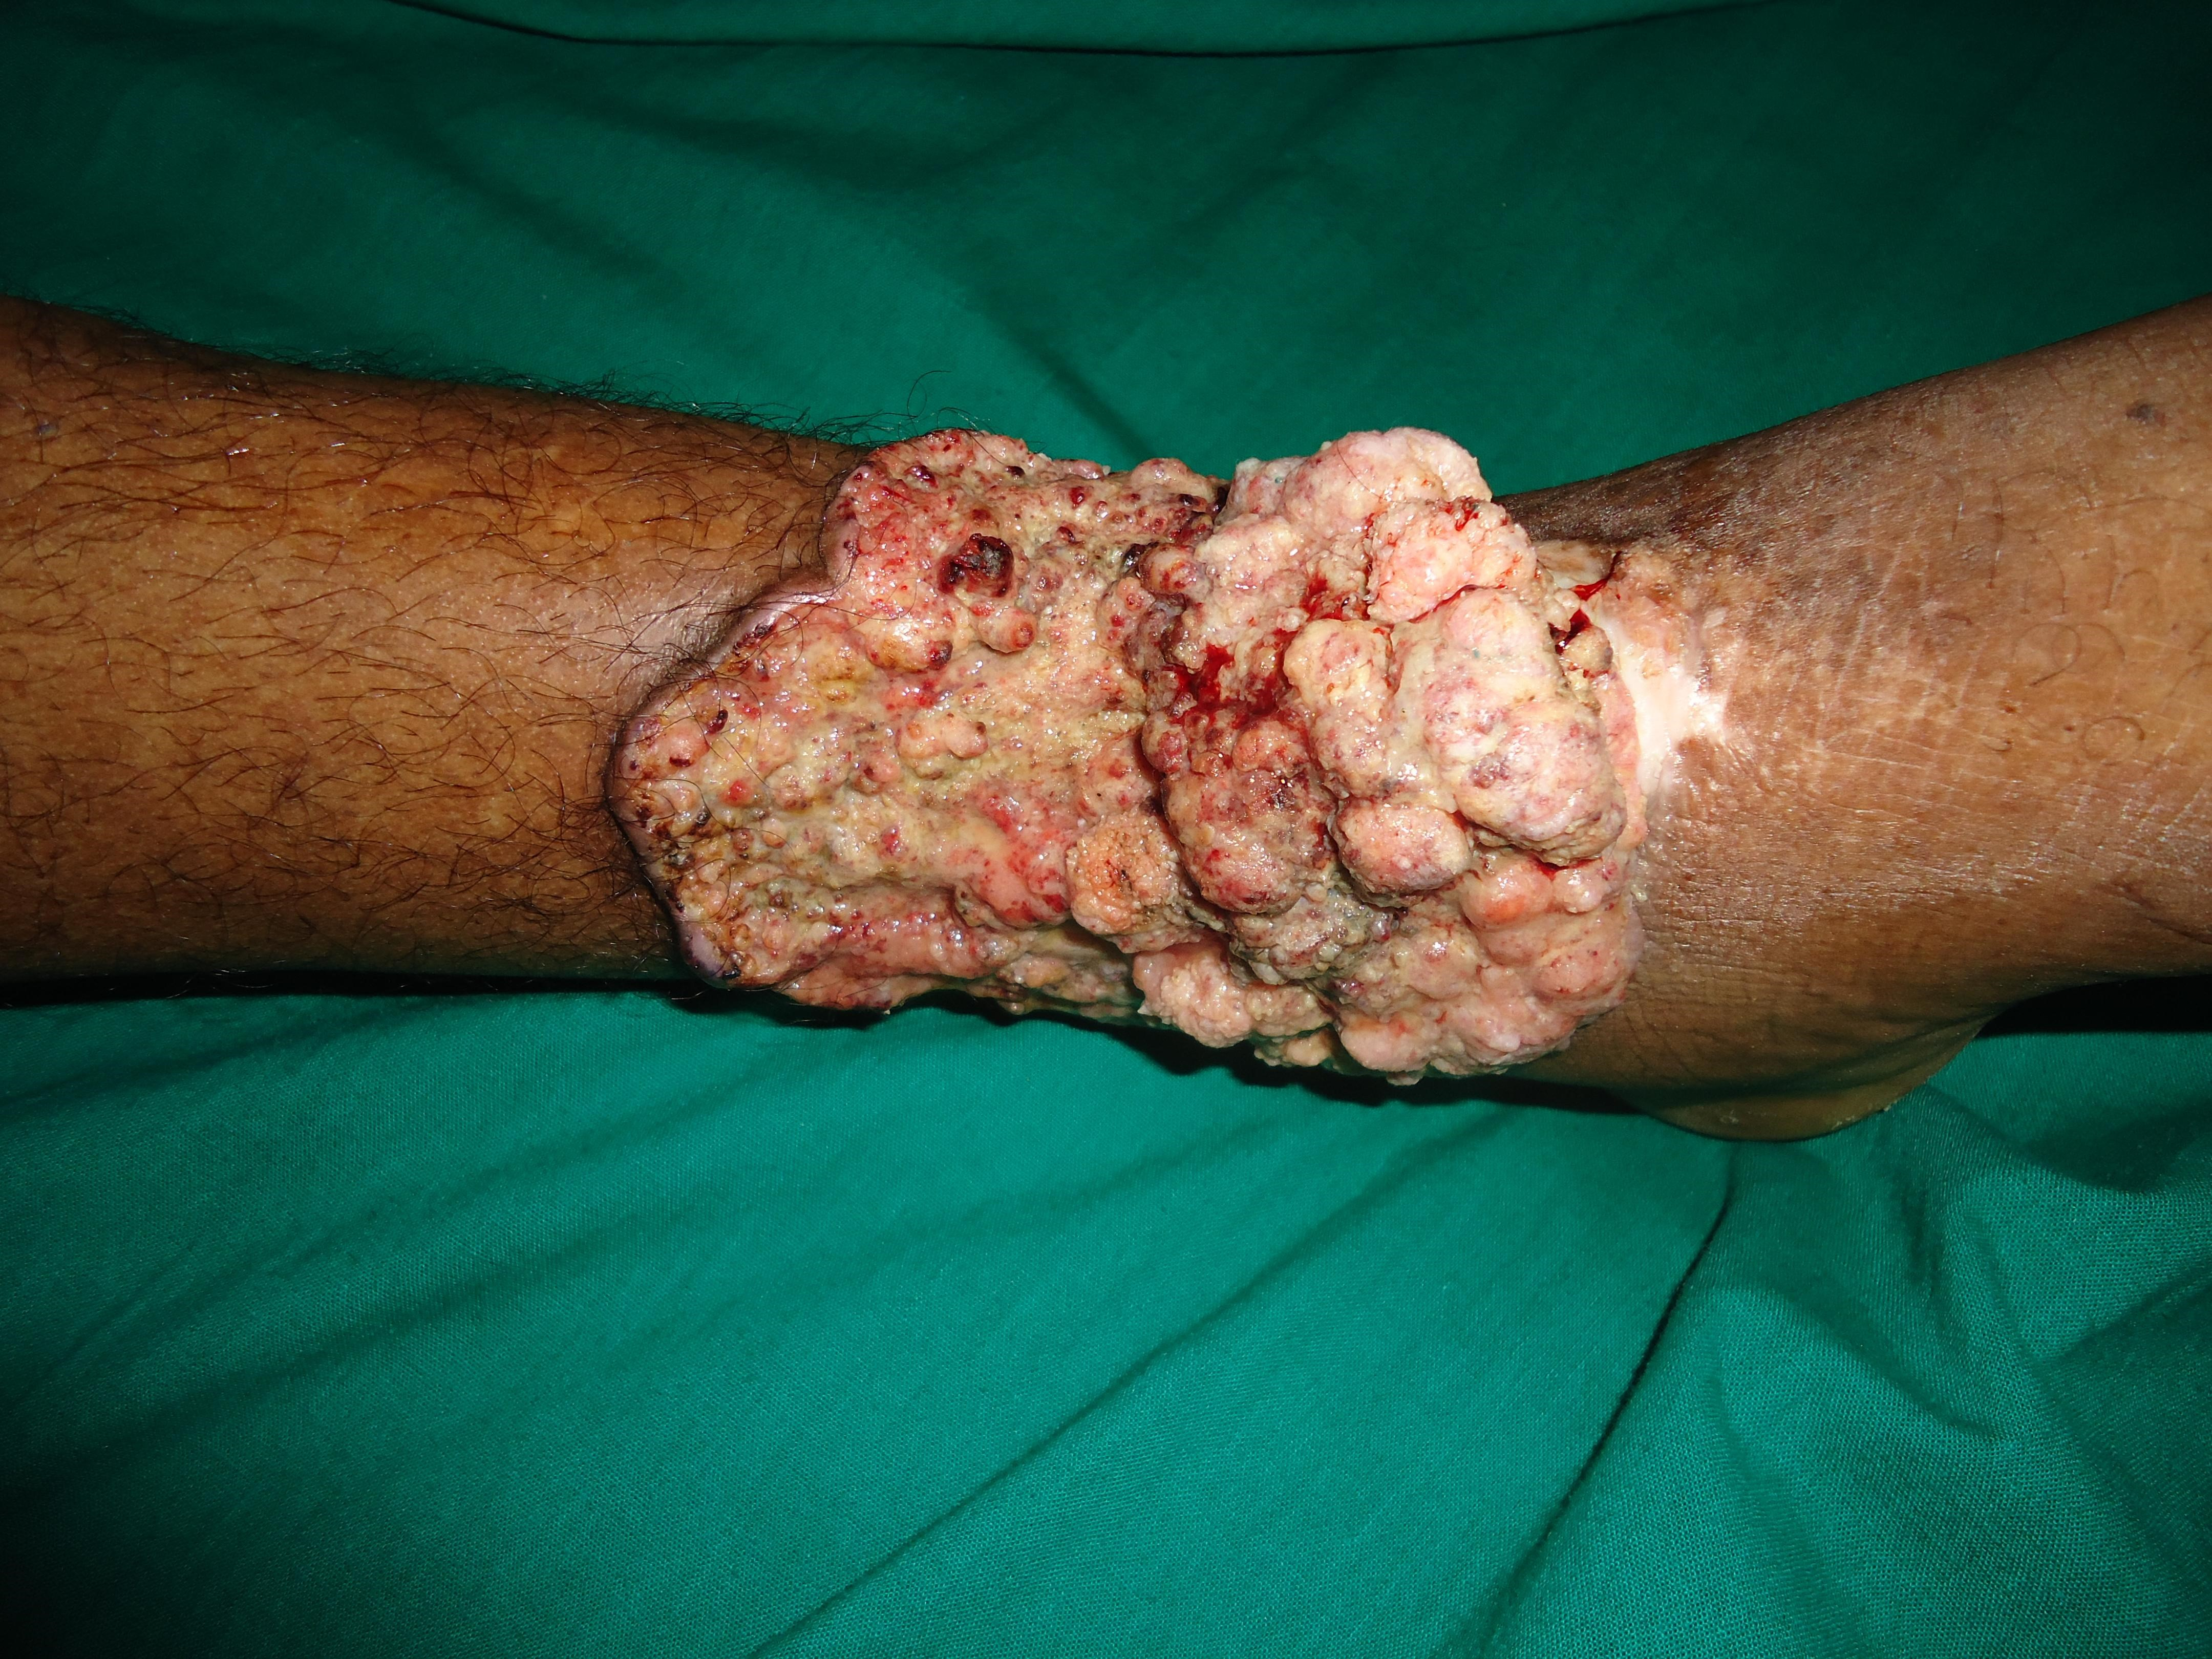
\includegraphics[width=0.45\textwidth]{images/sd260_scc.jpg}}}
	\end{tabular}
	\caption{Example images from the SD-260 dataset~\citep{yang2019self}.}
	\label{fig:sd260_examples}
\end{figure}

The four skin lesion datasets used in this study were intentionally restricted to a set of seven diagnostic categories to facilitate DL experiments. XXX Add motivation: why seven, why the specific seven chosen? For example, vascular lesions were excluded from the ISIC 2019 dataset, and classes such as angioma and solar lentigo were excluded from the Tayside dataset because they were not represented well in the other two datasets. The ISIC 2019, SD-260, Tayside, and Forth Valley data subsets used thus contained 25078, 13814, 2218, and 1518 images, respectively (Table~\ref{tab:generalisation_datasets}).

\begin{table}[h]
	\centering
	\caption{Number of images per diagnosis in each dataset.}
	\label{tab:generalisation_datasets}
	\resizebox{\textwidth}{!}{%
		\begin{tabular}{|ll|l|l|l|l|}
			\hline
			&                             & \textbf{ISIC 2019} & \textbf{SD-260} & \textbf{Tayside} & \textbf{Forth Valley} \\ \hline
			\multicolumn{1}{|l|}{\textbf{Benign}} & Actinic keratosis (B52)     & 867                & 1434            & 414              & 144                   \\
			\multicolumn{1}{|l|}{}                & Dermatofibroma (X9002)      & 239                & 303             & 56               & 78                    \\
			\multicolumn{1}{|l|}{}                & Naevus, melanocytic (X31z)  & 12875              & 1401            & 577              & 531                   \\
			\multicolumn{1}{|l|}{}                & Seborrhoeic keratosis (X01) & 2624               & 1133            & 538              & 290                   \\ \hline
			\multicolumn{1}{|l|}{\textbf{Malignant}} &
			\begin{tabular}[c]{@{}l@{}}Melanoma (X41) / \\ Melanoma in situ (X40)\end{tabular} &
			4522 &
			7094 &
			78 &
			205 \\
			\multicolumn{1}{|l|}{} &
			\begin{tabular}[c]{@{}l@{}}Squamous cell carcinoma (X12) / \\ Squamous cell carcinoma in situ (X11)\end{tabular} &
			628 &
			17 &
			176 &
			91 \\
			\multicolumn{1}{|l|}{}                & Basal cell carcinoma (X20)  & 3323               & 2432            & 379              & 179                   \\ \hline
			\textit{\textbf{Total}}               & \textit{}                   & \textit{25078}     & \textit{13814}  & \textit{2218}    & \textit{1518}         \\ \hline
		\end{tabular}%
	}
\end{table}

\subsection{Training Parameters}
\label{subsec:generalisation_training}
Two methods for image classification using DL were employed for this study. The first was a convolutional neural network, specifically an EfficientNet architecture~\citep{tan2019efficient} with a compound coefficient of 7 and an additional fully connected layer of 512 neurons preceding the output layer. The second was a SWIN-B transformer~\citep{liu2021swin}, a state-of-the-art visual transformer network for image classification. 

Subsequent training sessions each ran for 40 epochs, saving the model each time the lowest validation loss so far was achieved. Weights were optimised using stochastic gradient descent with batches of 16 images and a triangular2 cyclical scheduler~\citep{smith2017cyclical}, altering the learning rate between 10-5 and 10-2 and the momentum between 0.8 and 0.9. All images were pre-processed by cropping, resizing to 224 x 224 pixels, and normalising the pixel values between 0.0 and 1.0. Data augmentation was used to improve generalisation, specifically using a range of geometric and photometric transformations applied randomly when sampled. The full list of augmentations is…

Given an image, the deep network models predict class probabilities for each of the seven diagnostic classes. These probabilities are constrained, by definition, to sum to one. Three of the seven classes represent malignant lesions. By summing the probabilities of these three classes we obtain the probability that the observed lesion is malignant if the class probabilities computed are well-calibrated~\citep{carse2022calibration}. We adopted this rule to evaluate the ability of the CNN and SWIN transformer models to identify malignant lesions. Specifically, we used ROC curves to quantify the sensitivity-specificity trade-offs that can be obtained on our macroscopic image datasets. Models were pretrained on SD-260 data and then trained on either Tayside or Forth Valley data.

\subsection{Experiment Setup}
\label{subsec:generalisation_experiment}
We first evaluated the ability of the models to classify lesion images from each dataset after training on images from that same dataset. When using the larger datasets, ISIC 2019 and SD-260, we split each into disjoint training (60\%), validation (20\%) and test (20\%) sets. These splits are static: all training and testing with the datasets use the same splits. Given the limited sized of the Tayside and Forth Valley datasets, we used 10-fold cross-validation to estimate performance; each fold had disjointed training (70\%), validation (20\%) and test (10\%) sets and was estimated by averaging the 10 test results. These splits were also static across each fold, so that each experiment over the folds used 100\% of the data across the folds with the same training and validation splits in each fold.

We then evaluated the cross-dataset performance, measuring the class-balanced accuracy of each model when tested on data from datasets not used for training the model. We trained deep classifiers pre-trained with ImageNet~\citep{deng2009imagenet} on data from each of the datasets and then tested them on each of the datasets. Training sets were identical in composition to those used in the internal data classification experiment.

We evaluated the effect of transfer learning between the dermatology datasets using CNN and SWIM transformer models. We emphasise that all models in our experiments were pre-trained on ImageNet. Further pre-training was then performed on dermatology datasets. Firstly, we evaluated the effect of transfer between the large ISIC 2019 and SD-260 datasets. Secondly, we investigated the effect of transfer when the target domains (test data) were Tayside and Forth Valley data. This involved the use of multi-dataset pre-training sequences. For example, pre-training on SD-260 data and then training on Forth Valley training data, denoted “(SD-260, Forth Valley)”; pre-training on ISIC 2019 data, then on SD-260 data, and finally on Tayside training data, denoted “(ISIC 2019, SD-260, Tayside)”.

\subsection{Results}
\label{subsec:generalisation_results}
Results

\begin{table}[h]
	\centering
	\caption{Class-balanced accuracy when training and testing on the various datasets.}
	\label{tab:generalisation_results}
	\resizebox{\textwidth}{!}{%
		\begin{tabular}{|l|l|l|l|l|l|}
			\hline
			& Training Data & ISIC 2019      & SD-260         & Tayside        & Forth Valley   \\ \hline
			\textbf{CNN}  & ISIC 2019     & \textbf{0.978} & 0.804          & 0.825          & 0.855          \\
			& SD-260        & 0.879          & \textbf{0.969} & 0.855          & 0.867          \\
			& Tayside       &                &                & \textbf{0.875} & 0.850          \\
			& Forth Valley  &                &                & 0.847          & \textbf{0.891} \\ \hline
			\textbf{SWIN} & ISIC 2019     & \textbf{0.979} & 0.813          & 0.825          & 0.868          \\
			& SD-260        & 0.870          & \textbf{0.980} & 0.867          & 0.878          \\
			& Tayside       &                &                & \textbf{0.875} & 0.859          \\
			& Forth Valley  &                &                & 0.849          & \textbf{0.902} \\ \hline
		\end{tabular}%
	}
\end{table}

\begin{table}[h]
	\centering
	\caption{Balanced class accuracy when CNN and Swin transformers are tested on Tayside and Forth Valley data after various multi-dataset training sequences. }
	\label{tab:generalisation_models}
	\resizebox{\textwidth}{!}{%
		\begin{tabular}{|l|l|l|l|}
			\hline
			& Training Datasets               & Tayside        & Forth Valley   \\ \hline
			CNN  & SD-260, ISIC 2019               & 0.832          & 0.860          \\
			& ISIC 2019, SD-260               & 0.850          & 0.868          \\
			& ISIC 2019, Tayside              & 0.880          & 0.875          \\
			& SD-260, Tayside                 & \textbf{0.890} & 0.870          \\
			& ISIC 2019, SD-260, Tayside      & 0.879          & 0.876          \\
			& ISIC 2019, Forth Valley         & 0.850          & 0.900          \\
			& SD-260, Forth Valley            & 0.861          & \textbf{0.907} \\
			& ISIC 2019, SD-260, Forth Valley & 0.852          & 0.904          \\ \hline
			SWIN & SD-260, ISIC 2019               & 0.830          & 0.868          \\
			& ISIC 2019, SD-260               & 0.863          & 0.877          \\
			& ISIC 2019, Tayside              & 0.881          & 0.884          \\
			& SD-260, Tayside                 & \textbf{0.891} & 0.891          \\
			& ISIC 2019, SD-260, Tayside      & 0.890          & 0.896          \\
			& ISIC 2019, Forth Valley         & 0.854          & 0.910          \\
			& SD-260, Forth Valley            & 0.867          & 0.914          \\
			& ISIC 2019, SD-260, Forth Valley & 0.859          & \textbf{0.916} \\ \hline
		\end{tabular}%
	}
\end{table}

\begin{figure}[h]
	\centering
	\captionsetup[subfigure]{singlelinecheck=false}
	\begin{tabular}{c}
		\subcaptionbox{\centering Testing on the Tayside dataset.}{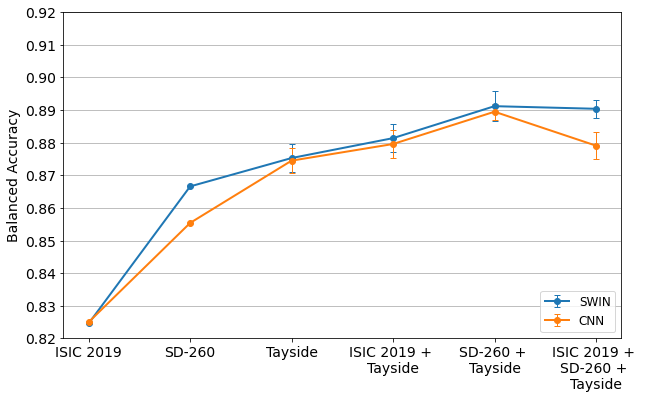
\includegraphics[width=0.9\textwidth]{images/tayside_model.png}} \\
		\subcaptionbox{\centering Testing on the Forth Valley dataset.}{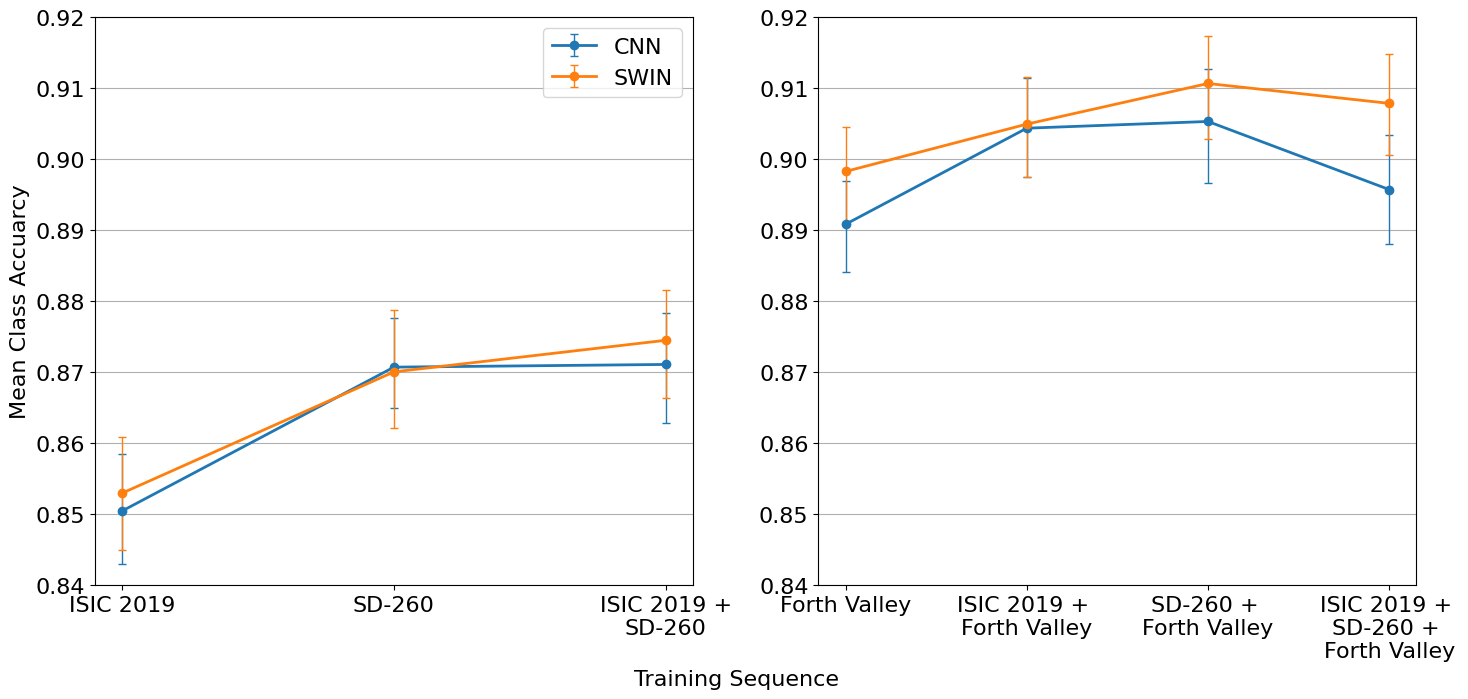
\includegraphics[width=0.9\textwidth]{images/forth_valley_model.png}}
	\end{tabular}
	\caption{Balanced accuracy of models when tested on Tayside and Forth Valley datasets after various pre-training sequences. Bars are +/- one standard error computed from the variance over cross-validation folds.}
	\label{fig:generalisation_models}
\end{figure}

\begin{figure}[h]
	\centering
	\captionsetup[subfigure]{singlelinecheck=false}
	\begin{tabular}{c}
		\subcaptionbox{\centering Testing on the Tayside dataset.}{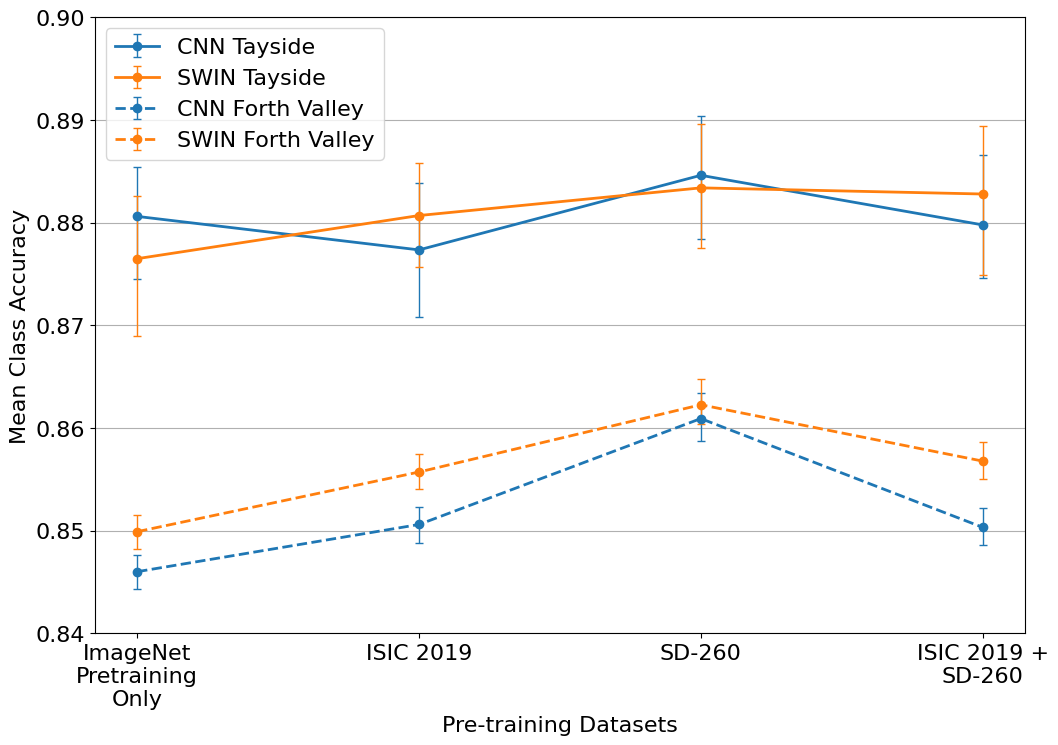
\includegraphics[width=0.9\textwidth]{images/tayside_testing.png}} \\
		\subcaptionbox{\centering Testing on the Forth Valley dataset.}{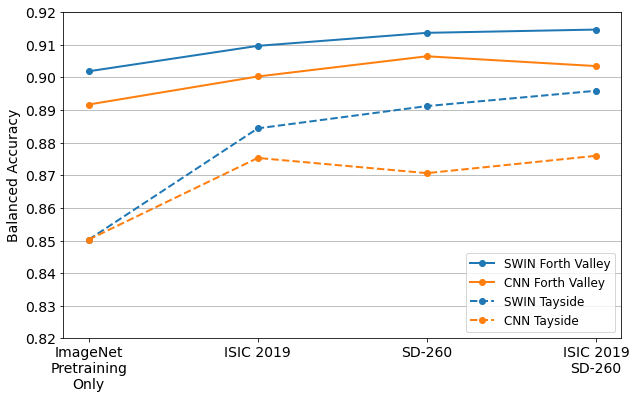
\includegraphics[width=0.9\textwidth]{images/forth_valley_testing.png}}
	\end{tabular}
	\caption{Balanced accuracy of the models demonstrating the performance of dataset cross-generalisation between the Tayside and Forth Valley datasets.}
	\label{fig:generalisation_testing}
\end{figure}

\begin{figure}[h]
	\centering
	\captionsetup[subfigure]{singlelinecheck=false}
	\begin{tabular}{c}
		\subcaptionbox{\centering Testing on the Tayside dataset.}{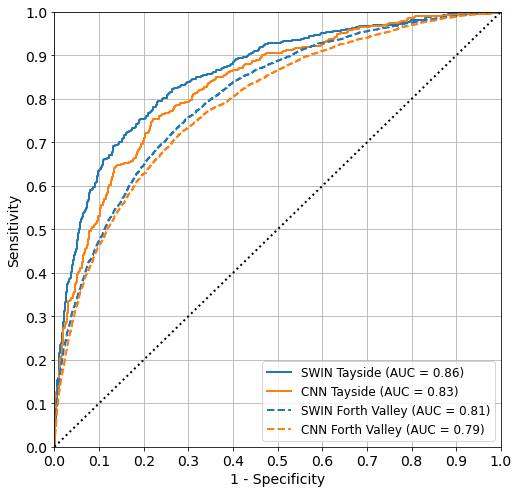
\includegraphics[width=0.85\textwidth]{images/tayside_roc.png}} \\
		\subcaptionbox{\centering Testing on the Forth Valley dataset.}{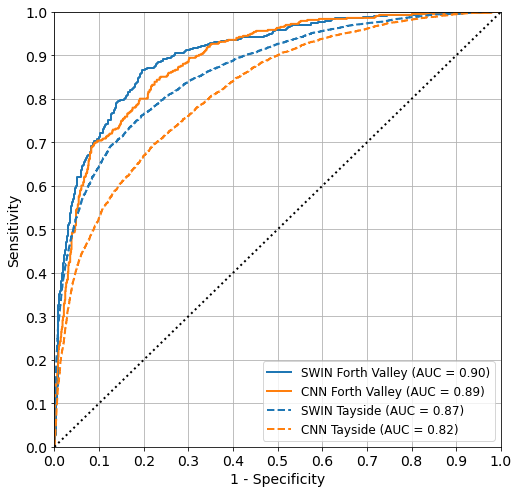
\includegraphics[width=0.85\textwidth]{images/forth_valley_roc.png}}
	\end{tabular}
	\caption{ROC curves for CNNs and SWIN transformers pre-trained on SD-260 prior to training on either Tayside or Forth Valley data.}
	\label{fig:generalisation_roc}
\end{figure}



\section{Generalisation Conclusion}
\label{sec:generalisation_conclusion}
Conclusion